% =====================================================================================
% BND School 2026 -- Z cross section from CMS Open Data: strategy, the three channels,
% and their combination.  Final deliverable of the combination subgroup.
%
% Build:  bash build.sh        (needs the cvmfs TeX Live 2025: metropolis, pgfopts, siunitx)
% Figures: ../output/plots/*.pdf  (vector, made by run_combination.py)
%          figures/*.pdf                      (vector, made by figures.py)
%          ../../z-mumu/output/v2/plots/*.png, ../../z-tautau/output/plots/*.png (channel plots)
%          figures/zee_*.png (pulled out of ../../z-ee/Zee_fit.tar.gz by figures.py)
% =====================================================================================
\documentclass[aspectratio=169,9pt,t]{beamer}
\usetheme[progressbar=frametitle,numbering=fraction,block=fill,sectionpage=none]{metropolis}

\usepackage{booktabs,amsmath,amssymb,graphicx,xcolor,tikz,array}
\usetikzlibrary{positioning,arrows.meta,shapes.geometric,fit,backgrounds,calc}
\usepackage[per-mode=symbol]{siunitx}

\graphicspath{{figures/}{../output/plots/}{../../z-mumu/output/v2/plots/}%
              {../../z-tautau/output/plots/}{../../z-tautau/slides/}}

% ------------------------------------------------------------------ palette (matches the figures)
\definecolor{mumu}{HTML}{2B6CB0}
\definecolor{tautau}{HTML}{EB811B}
\definecolor{ee}{HTML}{8E44AD}
\definecolor{comb}{HTML}{23373B}
\definecolor{good}{HTML}{14B03D}
\definecolor{warn}{HTML}{C0392B}
\setbeamercolor{alerted text}{fg=tautau}
\setbeamercolor{progress bar}{fg=mumu}
\setbeamercolor{progress bar in head/foot}{fg=mumu}
\setbeamercolor{frametitle}{bg=comb}
\setlength{\tabcolsep}{4pt}
\renewcommand{\arraystretch}{1.12}
\metroset{block=fill}
\setbeamersize{text margin left=5mm,text margin right=5mm}
\addtobeamertemplate{frametitle}{\vspace*{-1mm}}{\vspace*{-1mm}}

% ------------------------------------------------------------------ shortcuts
\newcommand{\Z}{\ensuremath{Z/\gamma^{*}}}
\newcommand{\mm}{\ensuremath{\mu\mu}}
\newcommand{\tauh}{\ensuremath{\tau_{\mathrm{h}}}}
\newcommand{\thth}{\ensuremath{\tauh\tauh}}
\newcommand{\muZ}{\ensuremath{\mu_{Z}}}
\newcommand{\ee}{\ensuremath{ee}}
\newcommand{\mll}{\ensuremath{m_{\ell\ell}}}
\newcommand{\pb}{\ensuremath{\,\mathrm{pb}}}
\newcommand{\sigll}{\ensuremath{\sigma(pp\to\Z\to\ell\ell,\ 60<\mll<120\,\mathrm{GeV})}}
\newcommand{\fig}[2][\textwidth]{\begin{center}\includegraphics[width=#1]{#2}\end{center}}
\newcommand{\src}[1]{{\scriptsize\color{gray}\texttt{#1}}}

\title{A combined \texorpdfstring{$Z$}{Z} cross section from CMS Open Data}
\subtitle{$Z\to\mu^{+}\mu^{-}$, $Z\to\tauh\tauh$ and $Z\to e^{+}e^{-}$, and what happens when you put them together}
\author{BND School 2026 -- combination subgroup\\[2pt]{\small Lieke Gijsen, Caspar van Eck}}
\date{16 September 2026}

\begin{document}

\begin{frame}[plain,noframenumbering]
\vspace{4mm}
{\color{gray}\footnotesize BND SCHOOL 2026 \quad\textbullet\quad COMBINATION SUBGROUP \quad\textbullet\quad
 LIEKE GIJSEN, CASPAR VAN ECK}\\[1.5mm]
{\color{comb}\rule{\textwidth}{0.8pt}}\\[3mm]
{\color{mumu}\LARGE\textbf{A COMBINED $Z$ CROSS SECTION FROM CMS OPEN DATA}}\\[2.5mm]
{\large $Z\to\mu^{+}\mu^{-}$, $Z\to\tauh\tauh$ and $Z\to e^{+}e^{-}$ --- and what happens when you put them together}\\[1mm]
{\color{gray}\small 16 September 2026 \quad\textbullet\quad CMS Open Data 2016 G+H,
 $\sqrt{s} = \SI{13}{TeV}$, $L = \SI{16.4}{fb^{-1}}$}\\[4mm]
\begin{columns}[T]
\begin{column}{0.52\textwidth}\small
\textbf{The result}
\begin{itemize}\setlength\itemsep{1pt}
\item $\sigll = \mathbf{1980 \pm 32\pb}$ per lepton flavour
\item \alert{the three channels do not agree}: $\chi^{2}/\mathrm{ndf} = 9.67/2$, $p = 0.008$
\item $Z\to\ee$ sits $3.0\sigma$ above $Z\to\mm$ --- a \alert{fixable convention violation}
      in the $\ee$ fit, not physics (slide 4)
\item adding a second \emph{precise} channel finally buys something: $35 \to \SI{32}{pb}$,
      $11\,\%$ --- but the luminosity floor stands
\end{itemize}
\end{column}
\begin{column}{0.44\textwidth}\small
\textbf{This deck}
\begin{enumerate}\setlength\itemsep{1pt}
\item the result, and the problem with it
\item strategy: three channels, one shared contract
\item $Z\to\mm$, $Z\to\tauh\tauh$, $Z\to\ee$
\item how the combination is actually done
\end{enumerate}
\vspace{1mm}
{\footnotesize + backup: references, full breakdown, variations}
\end{column}
\end{columns}
\end{frame}

% =====================================================================================
\begin{frame}{The measurement at a glance}
\begin{columns}[T]
\begin{column}{0.51\textwidth}
\small
\textbf{Data.} CMS 2016 Open Data, Run2016G+H, NanoAODv9.\\
$\sqrt{s} = \SI{13}{TeV}$, $L = \SI{16393.381}{pb^{-1}} \pm 1.2\,\%$ (normtag).

\medskip
\textbf{Three independent measurements}, same luminosity, same simulation, same fitter
(TRExFitter v1.8.0), same nuisance-parameter names:
\begin{itemize}\setlength\itemsep{1pt}
\item \textcolor{mumu}{$Z\to\mu^{+}\mu^{-}$}: 10.4 M events, $\delta\sigma/\sigma = 1.8\,\%$
\item \textcolor{ee}{$Z\to e^{+}e^{-}$}: 6.3 M events, $\delta\sigma/\sigma = 1.9\,\%$
\item \textcolor{tautau}{$Z\to\thth$}: 21 k events, 80\,\% of them jet$\to$\tauh{} fakes,
      $\delta\sigma/\sigma = 12\,\%$
\end{itemize}

\medskip
\textbf{Combination.} Covariance (BLUE) of the three, with the shared systematics correlated
through the \texttt{Category} contract of \texttt{fitting/CONVENTIONS.md}.

\medskip
\textbf{The punchline:} the two \emph{precise} channels \alert{disagree by $3.0\sigma$}, and we can
say exactly why. Everything else on this slide is downstream of that.
\end{column}

\begin{column}{0.47\textwidth}
\vspace{-2mm}
\begin{block}{Result}
\centering
$\sigll = \mathbf{1980 \pm 32}\pb$\\[3pt]
{\footnotesize $= 1980 \pm 0.5\,(\text{stat}) \pm 22\,(\text{syst}) \pm 7\,(\text{acc})
 \pm 21\,(\text{lumi})\pb$}\\[4pt]
{\footnotesize per lepton flavour, assuming lepton universality}\\[4pt]
{\footnotesize\color{warn}\textbf{channel compatibility
 $\chi^{2}/\mathrm{ndf} = 9.67/2$, $p = 0.008$}}
\end{block}
\begin{alertblock}{Read this with it}
{\footnotesize The $Z\to\ee$ fit lets a $\pm5.9\,\%$ theory \emph{normalisation} of its own signal
template float against its signal strength --- forbidden by \texttt{CONVENTIONS.md} \S3 precisely
because the two are degenerate. Correcting only that moves the combination by $-\SI{99}{pb}$.
\textbf{Slide 4.}}
\end{alertblock}
\vspace{-1mm}
{\footnotesize Without $\ee$: $1931 \pm 35\pb$, $p = 0.54$. CMS measures
$1952 \pm 4 \pm 18 \pm 45\pb$ (\href{https://arxiv.org/abs/2408.03744}{SMP-20-004}).}
\end{column}
\end{columns}
\end{frame}

% =====================================================================================
\section{1.\quad Result}

\begin{frame}{The combined cross section}
\vspace{-1mm}
\fig[0.58\textwidth]{forest.pdf}
\vspace{-3mm}
\begin{columns}[T]
\begin{column}{0.49\textwidth}\footnotesize
Weights: $\mu\mu$ $+0.596$, $\ee$ $+0.404$, $\tau\tau$ $-0.0003$. The $\tau\tau$ weight is negative
--- normal BLUE behaviour once $\rho$ exceeds the ratio of the uncertainties --- and it moves the
central value by \SI{0.06}{pb}.
\end{column}
\begin{column}{0.49\textwidth}\footnotesize
\alert{$\chi^{2}/\mathrm{ndf} = 9.67/2$, $p = 0.008$.} With two channels this was $1.70/1$
($p=0.19$) and could be waved through; with three it is a real test and it \emph{fails}.
$\ee$ and $\mu\mu$ are \SI{123}{pb} apart at $1.9\,\%$ and $1.8\,\%$ precision. No PDG scale
factor has been applied to hide it.
\end{column}
\end{columns}
\end{frame}

\begin{frame}{Why $Z\to\ee$ and $Z\to\mu\mu$ disagree --- and it is not physics}
\vspace{-3mm}
\fig[0.86\textwidth]{zee_normalisation.pdf}
\vspace{-4mm}
\begin{columns}[T]
\begin{column}{0.49\textwidth}\footnotesize
\texttt{CONVENTIONS.md} \S3: the signal theory templates must \textbf{vary the $C$ factor only,
renormalised to a constant yield}. $\mu\mu$ and $\tau\tau$ do; $\ee$ builds
\texttt{PDF}/\texttt{QCDScale} as raw LHE weight envelopes, so \texttt{QCDScale} carries the
$\pm5.87\,\%$ uncertainty of the aMC@NLO \emph{total cross section} as a normalisation on the
signal --- exactly degenerate with the POI.
\end{column}
\begin{column}{0.49\textwidth}\footnotesize
The fit pulls it to $-1.88\sigma$: it rescales the \emph{prediction} by $\kappa = 0.893$, and
\texttt{mu\_signal} $= 1.0509$ is measured against \emph{that}. The yields say
$(N_{\text{data}}-N_{\text{bkg}})/N_{\text{sig}} = 0.9700$, and $\hat\mu\times$(response of every
NP) $= 0.9706$ --- closure to $0.05\,\%$. \textbf{The fix is one line in the $\ee$ notebook:}
divide each LHE replica by its own $\Sigma w$.
\end{column}
\end{columns}
\end{frame}

\begin{frame}{Why combining now buys something --- and where the floor still is}
\begin{columns}[T]
\begin{column}{0.56\textwidth}
\vspace{-2mm}
\fig[\textwidth]{precision_budget.pdf}
\end{column}
\begin{column}{0.42\textwidth}\small
$Z\to\mm$ alone: $1931 \pm 35.4\pb$.\\
$\mu\mu \oplus \tau\tau$: $1931 \pm 35.4\pb$ --- \alert{$0.00\,\%$}.\\
All three: $1980 \pm 31.6\pb$ --- \alert{$10.7\,\%$}.

\medskip
\textbf{What changed.} $\tau\tau$ is nine times less precise, so it could never move the
uncertainty. $\ee$ is the first channel of \emph{comparable} precision, and that is exactly what
the previous round said was needed.

\medskip
\textbf{Why only $10.7\,\%$} and not the $29\,\%$ two independent equal measurements would give:
$\rho(\mu\mu,\ee) = 0.44$, almost all of it luminosity.

\medskip
\SI{21}{pb} of the \SI{32}{pb} is the luminosity: identical normtag value, identical runs,
identical $\pm1.2\,\%$ in all three channels. A fully correlated uncertainty cannot be combined
away. \textbf{The route to a better $Z$ cross section from this dataset is a better luminosity
calibration, not more channels.}
\end{column}
\end{columns}
\end{frame}

\begin{frame}{Where the uncertainty comes from}
\vspace{-3mm}
\fig[0.83\textwidth]{breakdown.pdf}
\vspace{-3mm}
{\footnotesize Left: contribution of each source to the combined uncertainty
($\delta_s = \sqrt{w^{T}C_{s}w}$); green = correlated between the channels. Right: the same
systematics as each channel's fit reports them. \texttt{Fit residual} (\SI{7.3}{pb}) is $\ee$-only:
the part of that channel's MINOS error its own grouped impacts do not add up to --- carried
uncorrelated, so its published total is reproduced exactly.}
\end{frame}

\begin{frame}{Lepton universality --- and what it is really telling us}
\vspace{-2mm}
\fig[0.88\textwidth]{universality.pdf}
\vspace{-2mm}
\begin{columns}[T]
\begin{column}{0.5\textwidth}\footnotesize
The combination \emph{assumes} universality, so it cannot test it. The ratios can --- and in a
ratio every $\rho = 1$ source cancels exactly: luminosity, pileup, L1 prefiring and the shared
PDF/scale/shower terms.
\\[3pt]
$R(\tau\tau/\mu\mu) = 1.08 \pm 0.13$, $+0.6\sigma$. It was $1.21 \pm 0.17$ before $\tau\tau$ moved
to DeepTau Tight in v3 --- exactly the shift that channel predicted.
\end{column}
\begin{column}{0.48\textwidth}\footnotesize
$R(\ee/\mu\mu) = 1.064 \pm 0.021$, \alert{$+3.0\sigma$}. Because so much cancels, the ratio is the
\emph{sharpest} statement that the two fits disagree --- which is why we quote it as a consistency
check between channels and \textbf{not} as a limit on $e$--$\mu$ universality. With the $\ee$
normalisation corrected it becomes $0.949 \pm 0.019$, $-2.7\sigma$: the disagreement changes sign,
so ``just apply the correction'' is not the answer either. A clean $\ee$ re-run is.
\end{column}
\end{columns}
\end{frame}

\begin{frame}{Each channel against the published measurement of the same decay}
\vspace{-2mm}
\fig[0.72\textwidth]{comparison_channels.pdf}
\vspace{-3mm}
\begin{columns}[T]
\begin{column}{0.49\textwidth}\footnotesize
\alert{Read the first two rows together.} Each of our two \emph{precise} channels agrees with the
ATLAS measurement of the same decay at the $1\sigma$ level --- $\mu\mu$ $-1.1\sigma$,
$\ee$ $+0.5\sigma$ --- and yet they disagree with \emph{each other} by $3.0\sigma$. No
contradiction: ATLAS's per-channel uncertainty is $\pm\SI{60}{pb}$, ours are $\pm35$ and
$\pm\SI{40}{pb}$.
\end{column}
\begin{column}{0.49\textwidth}\footnotesize
\textbf{Agreement with a published number is not a validation at this precision.} Everything is on
our window: ATLAS quotes $66$--$\SI{116}{GeV}$ and is scaled by $\sigma(60$--$120)/\sigma(66$--$116)
= 1.0143$ from the same aMC@NLO sample. CMS SMP-20-004 fits $ee$ and $\mu\mu$ \emph{together} and
publishes no per-channel number, so ATLAS is the only 13 TeV measurement that can carry this plot.
$\tau\tau$: CMS \href{https://arxiv.org/abs/1801.03535}{1801.03535}, five final states, same window.
\end{column}
\end{columns}
\end{frame}

\begin{frame}{Comparison with published measurements}
\vspace{-1mm}
\fig[0.58\textwidth]{comparison.pdf}
\vspace{-2mm}
{\footnotesize
Agreement with the CMS measurement of exactly the same quantity is within $0.5\sigma$ --- but so is
the $\mu\mu\oplus\tau\tau$ value ($1931\pb$, $0.4\sigma$) and nearly so the normalisation-corrected
one ($1882\pb$, $1.2\sigma$). \textbf{At this precision agreement with a published number does not
discriminate between our three readings and must not be used to pick one.} Both published numbers
carry a \emph{larger} relative luminosity uncertainty than we do (2.3\,\% and 2.1\,\% against
1.2\,\%) --- they are early-Run-2 measurements, while the 2016 G+H normtag luminosity is well
measured. Note this is not a fully independent check: the same NNLO reference
($\sigma_{DY} = \SI{6077.22}{pb}$) normalises the simulation behind all three of our $C$ factors.}
\end{frame}

% =====================================================================================
\section{2.\quad Strategy}

\begin{frame}{How the four pieces fit together}
\vspace{-2mm}
\begin{center}
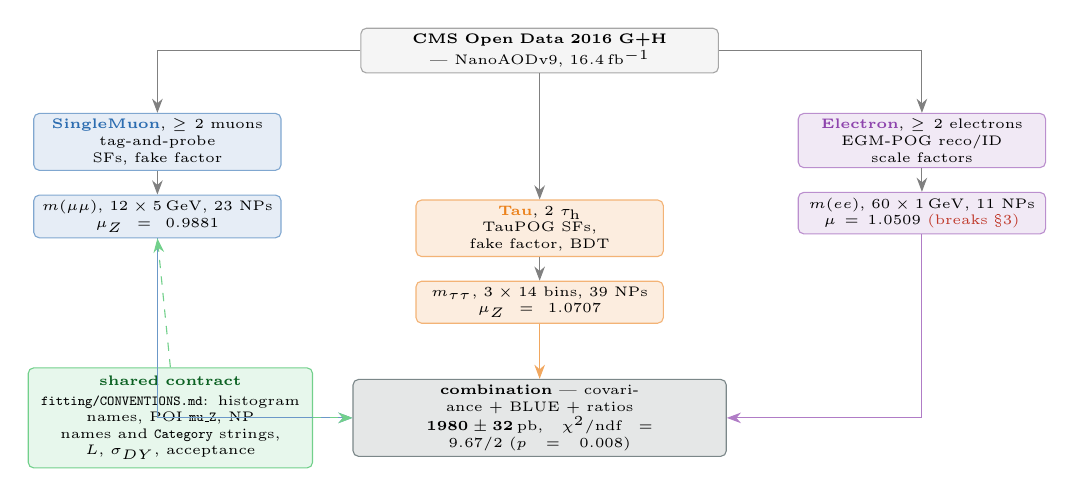
\begin{tikzpicture}[
  font=\tiny, node distance=3mm, >={Stealth[length=1.8mm]},
  box/.style={draw=black!35, rounded corners=2pt, fill=black!4, minimum height=5mm,
              text width=30mm, align=center, inner sep=2pt},
  mubox/.style={box, fill=mumu!12, draw=mumu!60},
  eebox/.style={box, fill=ee!12, draw=ee!60},
  taubox/.style={box, fill=tautau!14, draw=tautau!60},
  cbox/.style={box, fill=comb!12, draw=comb!60, text width=46mm},
  shared/.style={draw=good!60, fill=good!10, rounded corners=2pt, text width=34mm,
                 align=center, inner sep=3pt, font=\tiny}]

\node (data) [box, text width=44mm] {\textbf{CMS Open Data 2016 G+H} --- NanoAODv9, $\SI{16.4}{fb^{-1}}$};

\node (mu1) [mubox, below left=5mm and 10mm of data]
  {\textcolor{mumu}{\textbf{SingleMuon}}, $\ge2$ muons\\tag-and-probe SFs, fake factor};
\node (ee1) [eebox, below right=5mm and 10mm of data]
  {\textcolor{ee}{\textbf{Electron}}, $\ge2$ electrons\\EGM-POG reco/ID scale factors};
\node (ta1) [taubox, below=16mm of data]
  {\textcolor{tautau}{\textbf{Tau}}, 2 \tauh\\TauPOG SFs, fake factor, BDT};

\node (mu2) [mubox, below=of mu1] {$m(\mu\mu)$, $12\times\SI{5}{GeV}$, 23 NPs\\$\muZ = 0.9881$};
\node (ee2) [eebox, below=of ee1] {$m(ee)$, $60\times\SI{1}{GeV}$, 11 NPs\\$\mu = 1.0509$ \textcolor{warn}{(breaks \S3)}};
\node (ta2) [taubox, below=of ta1] {$m_{\tau\tau}$, $3\times14$ bins, 39 NPs\\$\muZ = 1.0707$};

\node (comb) [cbox, below=7mm of ta2] {\textbf{combination} --- covariance + BLUE + ratios\\%
  $\mathbf{1980 \pm 32\pb}$,\quad $\chi^{2}/\mathrm{ndf} = 9.67/2$ ($p = 0.008$)};

\node (sh) [shared, left=5mm of comb] {\textcolor{good!55!black}{\textbf{shared contract}}\\[1pt]
  \texttt{fitting/CONVENTIONS.md}: histogram\\ names, POI \texttt{mu\_Z}, NP names and
  \texttt{Category} strings, $L$, $\sigma_{DY}$, acceptance};

\draw[->,black!50] (data) -| (mu1);  \draw[->,black!50] (data) -| (ee1);
\draw[->,black!50] (data) -- (ta1);
\foreach \a/\b in {mu1/mu2, ee1/ee2, ta1/ta2} \draw[->,black!50] (\a) -- (\b);
\draw[->,mumu!70] (mu2) |- (comb);   \draw[->,ee!70] (ee2) |- (comb);
\draw[->,tautau!70] (ta2) -- (comb);
\draw[->,good!60,dashed] (sh.north) -- (mu2.south);
\draw[->,good!60,dashed] (sh.east) -- (comb.west);
\end{tikzpicture}
\end{center}
\vspace{-3mm}
{\footnotesize The \textcolor{good!60!black}{green} contract is what makes the combination
possible at all: because the channels name `\texttt{Lumi}', `\texttt{Pileup}',
`\texttt{L1Prefiring}', `\texttt{PDF}' \ldots{} identically and group them into the same
\texttt{Category}, the correlations can be assigned category by category instead of guessed. It is
also what tells us the $\ee$ channel has a problem: \textcolor{warn}{\S3} of the same contract is
the line its theory templates break.}
\end{frame}

\begin{frame}{Data and simulation}
\begin{columns}[T]
\begin{column}{0.52\textwidth}\footnotesize
\textbf{Collision data} (Run2016G+H only --- 16 of the 36\,\si{fb^{-1}} CMS recorded in 2016)
\begin{center}\scriptsize
\begin{tabular}{@{}llr@{}}
\toprule
dataset & recid & events \\ \midrule
\textcolor{mumu}{SingleMuon} G / H & 30530 / 30563 & 324 M \\
\textcolor{ee}{Electron} G / H & 30529 / 30562 & 232 M \\
\textcolor{tautau}{Tau} G / H & 30532 / 30565 & 156 M \\
\bottomrule
\end{tabular}
\end{center}
Certified with the 2016 golden JSON restricted to runs 278820--284044. The three \emph{selections}
are disjoint: the only process that can enter two of them is $ZZ\to4\ell$, 61 of the 10.4 M
$\mu\mu$ events ($0.0006\,\%$), so the data statistics are uncorrelated as a fact (backup).

\medskip
\textbf{Luminosity.} $L = \SI{16393.381}{pb^{-1}}$, the \emph{normtag} value from CMS Open Data
record 1059. An earlier \texttt{brilcalc} call without \texttt{-{}-normtag} gave
\SI{16290.713}{pb^{-1}}, 0.63\,\% low; all three channels use the normtag value, which is why the
luminosity is \emph{exactly} correlated between them --- and at $1.2\,\%$ it is better than the
$2.3\,\%$ CMS and $2.1\,\%$ ATLAS carry.
\end{column}

\begin{column}{0.46\textwidth}\footnotesize
\textbf{Simulation} (UL16 postVFP, streamed from EOS or read from dCache)
\begin{center}\scriptsize
\begin{tabular}{@{}lll@{}}
\toprule
sample & recid & used for \\ \midrule
DY M-50 aMC@NLO & 35669 & signal, all three \\
DY M-50 madgraph & 35671 & generator syst. \\
DY M-10to50 & 35631 & $\tau\tau$ background \\
$t\bar t$, $tW$, $VV$, $W$+jets & --- & backgrounds \\
\bottomrule
\end{tabular}
\end{center}
\textbf{Normalisation.} $\sigma(\Z\to\ell\ell,\ m > \SI{50}{GeV}) = \SI{6077.22}{pb}$ (NNLO). Each
channel's \muZ{} multiplies the LHE-flavour slice of it inside $60 < m_{\mathrm{LHE}} < 120$:
\begin{center}\scriptsize
\begin{tabular}{@{}lr@{}}
\toprule
$\sigma^{\text{pred}}(60$--$120)$ & \\ \midrule
$\ee$ & \SI{1954.1}{pb} \\
$\mu\mu$ & \SI{1953.9}{pb} \\
$\tau\tau$ & \SI{1944.9}{pb} \\
\bottomrule
\end{tabular}
\end{center}
The 0.47\,\% spread is the generator's flavour shares (the $\tau$ mass is in the matrix element),
not a definition --- which is why we combine \emph{cross sections}, never \muZ{} (backup).
\end{column}
\end{columns}
\end{frame}

% =====================================================================================
\section{3.\quad The three channels}

\begin{frame}{$Z\to\mu^{+}\mu^{-}$: a 1.8\,\% measurement with 10 million events}
\begin{columns}[T]
\begin{column}{0.46\textwidth}\footnotesize
\textbf{Selection.} \texttt{HLT\_IsoMu24 || HLT\_IsoTkMu24}; exactly two tight, isolated,
opposite-sign muons, $p_{T} > 26/20\,$GeV, $|\eta| < 2.4$, $60 < m(\mm) < \SI{120}{GeV}$; FSR
photons recovered from the \texttt{FsrPhoton} collection.

\medskip
\textbf{Corrections, all measured in this data.}
\begin{itemize}\setlength\itemsep{0pt}
\item ID / isolation / trigger scale factors from tag-and-probe \emph{fits} on the $Z$ peak
      (20 M pairs), with trigger-object matching
\item pileup weights from the Open Data luminosity table, L1-prefiring weights
\item $Z$-peak muon momentum calibration per $|\eta|$ bin
\item non-prompt muons from a same-sign fake factor (3.8 k events, 0.04\,\% of the yield)
\end{itemize}

\medskip
\textbf{Backgrounds} are tiny: 69 k of 10.4 M events (0.66\,\%), dominated by $t\bar t$ (32 k) and
$Z\to\tau\tau$ (11 k).
\end{column}

\begin{column}{0.52\textwidth}
\vspace{-3mm}
\fig[0.72\textwidth]{datamc_SR_mass_fit_log.png}
\vspace{-3mm}
{\scriptsize The distribution that is fitted, shown in \SI{1}{GeV} input bins; the fit runs in
$12 \times \SI{5}{GeV}$. Note the ratio panel --- data sit 3--4\,\% below the prediction at
$62$--$\SI{78}{GeV}$. That deficit is the reason the next slide exists.}
\end{column}
\end{columns}
\end{frame}

\begin{frame}{$Z\to\mu\mu$: which number to take --- the channel's review, and its repair}
\begin{columns}[T]
\begin{column}{0.54\textwidth}
\vspace{-3mm}
\fig[\textwidth]{mumu_fit_stability.pdf}
\end{column}
\begin{column}{0.44\textwidth}\footnotesize
The channel's own review (\src{z-mumu/REVIEW.md}, F3/F4) found the 30-bin shape fit
\alert{not robust}: \muZ{} moved over $0.990$--$1.006$, because the only template that could
absorb a 3--4\,\% data deficit at 62--\SI{78}{GeV} was \texttt{SigModel} --- and that template
mixed the generator comparison with a phase-space artefact (the powheg sample is generated with
$m_{\mathrm{LHE}} < \SI{120}{GeV}$, depleting its two highest bins by 10\,\% and 33\,\%).

\medskip
\textbf{The channel fixed both.} Fit in $12\times\SI{5}{GeV}$ bins so the shape parameters are not
over-constrained, no smoothing, MINOS everywhere; \texttt{SigModel} rebuilt with both generators
inside a common $50 < m_{\mathrm{LHE}} < \SI{120}{GeV}$ window and mirrored.

\medskip
\textbf{We therefore take the shape fit:} $\muZ = 0.9881 \pm 0.0159$, GoF $p = 0.79$, stable to
$\pm0.2\,\%$ across the binnings that describe the data. The $\pm0.7\,\%$ lineshape term the
review had asked for as a stop-gap is \alert{retired} --- the two-sided template carries it inside
the fit. Counting instead would move the combination by $+\SI{11.2}{pb}$: reported as a variation,
not used.
\end{column}
\end{columns}
\end{frame}

\begin{frame}{$Z\to\tauh\tauh$: a 12\,\% measurement where 80\,\% of the data is background}
\begin{columns}[T]
\begin{column}{0.46\textwidth}\footnotesize
\textbf{Selection.} Double-$\tauh$ trigger (different path in G and H), both legs HLT-matched;
two opposite-sign \tauh{} with $p_{T} > \SI{40}{GeV}$, $|\eta| < 2.1$, decay modes 0/1/10/11,
DeepTau2017v2p1 \textbf{Tight} vs jets (v3 --- the working point v2.1 recommended and v3 adopted);
$e$/$\mu$ veto keeps it orthogonal to the other two channels.
$\Rightarrow$ 21 160 events, of which \alert{$\sim$64\,\% are jets faking a \tauh}.

\medskip
\textbf{No QCD simulation is used.} The fake background comes from data: a fake factor
$\mathrm{FF}(\text{era}, \mathrm{DM}, N_{\text{jets}}, p_{T})$ measured in a same-sign region and
applied to opposite-sign events whose leading \tauh{} fails Tight, times an OS/SS correction
of 1.04--1.15 measured per (era, $N_{\text{jets}}$, BDT category), with the genuine-$\tau$ MC
subtracted. A $k$-fold BDT (held-out AUC 0.966) splits the signal region into \alert{three
categories} by purity.

\medskip
\textbf{Mass.} The visible di-$\tau$ mass is not a $Z$ mass. A per-event likelihood over the
$\tau$ visible-energy fractions using the MET covariance gives $m_{\tau\tau}$ with scale 0.99 and
resolution 11\,\% (against 0.80 / 13\,\% for $m_{\text{vis}}$).
\end{column}

\begin{column}{0.52\textwidth}
\vspace{-3mm}
\fig[0.62\textwidth]{fit_SR2_postfit.png}
\vspace{-3mm}
{\scriptsize Post-fit $m_{\tau\tau}$ in the most signal-like BDT category (score $> 0.90$);
the fit runs over all three, 14 bins each, 0--\SI{350}{GeV}. Pink = the data-driven
jet$\to$\tauh{} fakes, orange = $Z\to\tau\tau$. Counting over the whole signal region instead
gives \SI{2173}{pb}: it is the low-score categories that fix the fake normalisation.}
\end{column}
\end{columns}
\end{frame}

\begin{frame}{$Z\to\tauh\tauh$: result and what limits it}
\begin{columns}[T]
\begin{column}{0.44\textwidth}\footnotesize
\begin{center}\small
$\muZ = 1.071\,^{+0.114}_{-0.100}$\\[2pt]
$\sigma(60$--$120) = 2082 \pm 41\,^{+222}_{-194} \pm 76\pb$\\[2pt]
{\footnotesize goodness of fit $p = 0.25$}
\end{center}

\medskip
\begin{center}\scriptsize
\begin{tabular}{@{}lr@{}}
\toprule
source & impact on \muZ \\ \midrule
$\tauh$ ID & 8.4\,\% \\
fakes (fake factor) & \phantom{0}6.5\,\% \\
MC statistics & \phantom{0}3.9\,\% \\
$\tauh$ trigger & \phantom{0}3.0\,\% \\
background normalisation & \phantom{0}2.6\,\% \\
$\tauh$ energy scale & \phantom{0}1.5\,\% \\
signal modelling (PDF, scales, PS) & \phantom{0}1.3\,\% \\
luminosity & \phantom{0}0.7\,\% \\
\alert{data statistics} & \alert{\phantom{0}2.1\,\%} \\
\bottomrule
\end{tabular}
\end{center}

\smallskip
Acceptance $A = 0.23\,\%$ with a 3.7\,\% uncertainty --- the double \SI{40}{GeV} cut on the
\emph{visible} $\tau$ momentum sits on the $Z$ $p_{T}$ tail, where the QCD scale dependence is
3.4\,\%.
\end{column}

\begin{column}{0.54\textwidth}
\vspace{-3mm}
\fig[0.88\textwidth]{step3_fakefactors.png}
\vspace{-3mm}
{\scriptsize The fake factors, binned in era, decay mode, $N_{\text{jets}}$ and $p_{T}$. Without
the $N_{\text{jets}}$ binning the same-sign closure is off by 10--25\,\% per jet bin; without the
era binning by $\pm5\,\%$ (the HLT $\tau$ isolation changed between G and H).
\\[3pt]
Moving from DeepTau Medium (v2.1) to Tight (v3) took the channel from
$\muZ = 1.205$, $\delta\sigma/\sigma = 14\,\%$ to $\muZ = 1.071$, $12\,\%$ --- and
$R(\tau\tau/\mu\mu)$ from $1.21 \pm 0.17$ to $1.08 \pm 0.13$.}
\end{column}
\end{columns}
\end{frame}

\begin{frame}{$Z\to e^{+}e^{-}$: 6.3 million events, and one line of the contract}
\begin{columns}[T]
\begin{column}{0.47\textwidth}\footnotesize
\textbf{Selection.} \texttt{HLT\_Ele27\_WPTight\_Gsf}; exactly two opposite-sign electrons,
$p_{T} > \SI{20}{GeV}$, $|\eta| < 2.5$, \texttt{cutBased} $\ge$ Medium;
$60 < m_{ee} < \SI{120}{GeV}$. $\Rightarrow$ \textbf{6 320 097} events, background
44.9 k ($0.7\,\%$): $t\bar t$ 21.6 k, diboson 13.2 k, $Z\to\tau\tau$ 6.7 k, $W$+jets 3.4 k.

\medskip
\textbf{Corrections.} Pileup, L1-prefiring, and EGM-POG reco + Medium-ID scale factors. DY is split
by LHE truth, so the $\tau\tau$ feed-down is a separate template. \alert{No trigger SF, no electron
energy scale, no FSR recovery, no charge-misID, no fake background} (backup).

\medskip
\textbf{Fit.} TRExFitter v1.8.0, $m_{ee}$ in $60\times\SI{1}{GeV}$ bins, one signal region,
11 NPs $+$ 60 $\gamma$. $\Rightarrow \mu = 1.0509 \pm 0.0202$,
$\sigma(60$--$120) = 2054 \pm 40\pb$. \alert{No goodness of fit was run} --- the only channel
without one.
\end{column}

\begin{column}{0.51\textwidth}
\vspace{-4mm}
\fig[0.48\textwidth]{zee_SR_postfit.png}
\vspace{-5mm}
\fig[0.80\textwidth]{zee_pulls.png}
\vspace{-4mm}
{\scriptsize \alert{\texttt{Pileup} at $-2.9\sigma$, \texttt{L1 prefiring} at $+3.6\sigma$} (off the
axis), \texttt{Electron ID} squeezed to $0.08$ of its input width: a shape mismatch absorbed by
calibration parameters in a 1 GeV binning. $z$-$\mu\mu$ fixed the same thing with \SI{5}{GeV} bins.}
\end{column}
\end{columns}
\end{frame}

% =====================================================================================
\section{4.\quad Combination}

\begin{frame}{What is combined, and how}
\begin{columns}[T]
\begin{column}{0.5\textwidth}\small
\textbf{The observable.} $\sigll$ per lepton flavour, \emph{assuming lepton universality}:
\[ \sigma_{c} = \hat\mu_{c}\times\sigma^{\text{pred}}_{c}(60\text{--}120) \]

\textbf{Not} $\muZ$ itself: the three channels normalise to references \SI{9}{pb} apart for the
same quantity (backup), so averaging the $\mu$'s would average three different things.

\medskip
\textbf{The covariance}, source by source,
\[ C = \sum_{s} C_{s},\qquad (C_{s})_{ij} = \rho_{s}\,s_{i}s_{j} \]
then standard BLUE,
\[ w = \frac{C^{-1}u}{u^{T}C^{-1}u},\quad \hat\sigma = w^{T}x,\quad
   \mathrm{Var} = \frac{1}{u^{T}C^{-1}u} \]
with $\chi^{2}$ (ndf\,=\,2 now) for compatibility, and the combined uncertainty decomposed as
$\delta_{s} = \sqrt{w^{T}C_{s}w}$.
\end{column}

\begin{column}{0.47\textwidth}\small
\textbf{Two details that are easy to get wrong.}

\smallskip
\emph{In-fit systematics scale with the prediction}, because \muZ{} multiplies a fixed number:
$\delta\sigma = s_{\text{group}}\times\sigma^{\text{pred}}$. \emph{The acceptance is
multiplicative}, $\delta\sigma = a\times\sigma^{\text{meas}}$, since $\sigma = \sigma_{\text{fid}}/A$
--- and $A$ is outside the $\mu\mu$ and $\tau\tau$ likelihoods (0.61\,\% and 3.7\,\%), so the
combination has to add it. The $\ee$ channel fits against the full $60$--$\SI{120}{GeV}$
prediction directly, so for it $A$ is \emph{inside} the fit and there is no separate term.

\smallskip
Because the acceptance is multiplicative, the BLUE is \emph{iterated}: the terms are re-evaluated
at the combined value until stable ($<\SI{0.1}{pb}$).

\medskip
\textbf{Cross-checked} against an explicit profile likelihood with one nuisance per shared source,
\[ -2\ln L = \sum_{c}\frac{(x_{c}-\sigma-\sum_{s}d_{cs}\theta_{s})^{2}}{u_{c}^{2}}
   + \sum_{s}\theta_{s}^{2} \]
which additionally carries the $\tau\tau$ channel's asymmetric error. Same answer:
$1980\,^{+31}_{-31}$ against $1980 \pm 32\pb$.
\end{column}
\end{columns}
\end{frame}

\begin{frame}{The correlation model --- the only judgement in the whole thing}
\vspace{-1mm}
\begin{columns}[T]
\begin{column}{0.55\textwidth}
\vspace{-3mm}
\fig[\textwidth]{sources.pdf}
\end{column}
\begin{column}{0.43\textwidth}\scriptsize
\textbf{$\rho = 1$ --- derived once, used by all}
\begin{itemize}\setlength\itemsep{0pt}
\item \texttt{Luminosity}: same normtag value, same runs, same $\pm1.2\,\%$
\item \texttt{Pileup}, \texttt{L1 prefiring}: same 2016 profile, same weights
\item \texttt{Background normalisation}: literally the same \texttt{XS\_*} parameters on the same
      MC samples
\item PDF, $\alpha_{s}$, QCD scale, PS: same Hessian members and the same 7-point envelope of the
      \emph{same} aMC@NLO sample
\end{itemize}

\smallskip
\textbf{$\rho = 0$ --- different objects, methods or events}
\begin{itemize}\setlength\itemsep{0pt}
\item muon vs electron vs $\tauh$ calibrations: no common input
\item \texttt{Gammas}: same sample, three \emph{disjoint} selections
\item fakes, MET; \texttt{Fit residual} ($\ee$ only)
\item data statistics: \emph{disjoint} primary datasets
\end{itemize}

\smallskip
\textbf{The split of \texttt{Signal modelling}.} Only $\mu\mu$ still fits a generator systematic
(powheg vs aMC@NLO, 0.4\,\% on \muZ); $\tau\tau$ dropped its LO-vs-NLO version in v2.1 and $\ee$
never had one. We still split the category and decorrelate the generator part --- so the
``\texttt{SigModel} correlated'' variation is exactly null.

\smallskip
$\Rightarrow$ $\rho(\mu\mu,\ee) = \mathbf{0.44}$ (almost all luminosity),
$\rho(\mu\mu,\tau\tau) = 0.13$, $\rho(\tau\tau,\ee) = 0.09$.
\end{column}
\end{columns}
\end{frame}

\begin{frame}{Cross-checks: the model is not what limits us --- one channel is}
\begin{columns}[T]
\begin{column}{0.53\textwidth}
\vspace{-2mm}
\fig[\textwidth]{variations.pdf}
\end{column}
\begin{column}{0.45\textwidth}
\vspace{-2mm}
\fig[\textwidth]{likelihood_scan.pdf}
\end{column}
\end{columns}
\vspace{-2mm}
{\footnotesize
The two rows that \emph{bracket the entire correlation model} span \SI{9.9}{pb}, under a third of
the total uncertainty, and every modelling choice inside that bracket moves the answer by less
than $0.4\sigma$. What dominates instead is \alert{\texttt{ee normfix} at $-\SI{98.5}{pb}$
($-3.1\sigma$)} --- a convention violation inside one channel --- and \texttt{no ee} at
$-\SI{49.2}{pb}$, the size of the $\ee$ contribution. Right: the profile likelihood and the BLUE
parabola lie on top of each other.}
\end{frame}

\begin{frame}[fragile]{What this is not, and what is left to do}
\begin{columns}[T]
\begin{column}{0.49\textwidth}\small
\begin{alertblock}{Not a TRExFitter MultiFit}
The channel workspaces are not all committed and were not rebuilt, so the shared nuisance
parameters are correlated through their \texttt{Category} totals rather than \emph{profiled
jointly}. The fitting is still TRExFitter's --- it produced all three inputs.
\end{alertblock}
The MultiFit config is generated and syntax-checked (\src{combination/fit/comb.config}); running
\src{fit/run\_multifit.py --dry-run} now prints what still blocks it:
{\scriptsize
\begin{verbatim}
POI: mu_Z           (z-ee: mu_signal)
Region: ee_SR       (z-ee: "SR")
Sample DYee, SIGNAL (z-ee: DY_ee, BACKGROUND)
Lumi, XS_WW/WZ/ZZ   (z-ee: LUMI, XS_VV)
PDF/QCDScale renormalised to a
  constant yield    (z-ee: raw envelopes)
\end{verbatim}}
\vspace{-2mm}
{\footnotesize This matters more than it used to: $\ee$ carries 40\,\% of the weight, and a joint
fit would expose the \texttt{QCDScale} problem \emph{structurally} instead of as a variation.}
\end{column}

\begin{column}{0.49\textwidth}\small
\textbf{What $Z\to ee$ has to change} (\src{combination/docs/01-inputs.md})
\begin{enumerate}\setlength\itemsep{0pt}
\item \alert{renormalise \texttt{PDF}/\texttt{QCDScale} to a constant yield} --- this is the whole
      \SI{99}{pb}
\item accumulate the envelopes per LHE flavour
\item adopt \texttt{CONVENTIONS.md} \S1--\S4 and publish a results JSON
\item run the saturated-model goodness of fit
\item fit in coarser bins than $60\times\SI{1}{GeV}$
\item smooth or merge \texttt{Wjets} (24\,\% MC stat., $\sim$30 floored bins)
\end{enumerate}
\emph{Already fixed on 16 Sep:} the reference cross section (their \SI{1954.1032}{pb} agrees with
ours to $4\times10^{-6}$) and the negative bins. Full list: \src{ASK\_Z\_EE.md}.

\medskip
\textbf{Inherited caveats we did not fix:} the $\mu\mu$ 60--\SI{80}{GeV} lineshape; prefiring,
muon and pileup calibrations all in-house; $\tau\tau$ v3 publishes only its nominal, so there are
no $\tau\tau$ cross-check rows.
\end{column}
\end{columns}
\end{frame}

\begin{frame}{Conclusions}
\begin{columns}[T]
\begin{column}{0.56\textwidth}
\begin{block}{}
\centering\large
$\sigll = \mathbf{1980 \pm 32}\pb$\\[3pt]
\normalsize $\chi^{2}/\mathrm{ndf} = \mathbf{9.67/2}$\;\; ($p = 0.008$)
\end{block}
\footnotesize
\begin{enumerate}\setlength\itemsep{3pt}
\item \textbf{Quote the compatibility with the value.} Three very different analyses of the same
      $\SI{16.4}{fb^{-1}}$, and the two \emph{precise} ones are \SI{123}{pb} apart.
\item \textbf{We know why, and it is fixable.} The $\ee$ fit lets a $\pm5.9\,\%$ theory
      \emph{normalisation} float against its own signal strength; \texttt{QCDScale} is pulled
      $-1.88\sigma$ and $\hat\mu$ is measured against a prediction the fit rescaled by 0.893.
      Correcting only that: $-\SI{99}{pb}$. \textbf{One line in the $\ee$ notebook.}
\item \textbf{Combining finally buys something}: $35 \to \SI{32}{pb}$, $11\,\%$ --- the first
      channel of precision comparable to $\mu\mu$ does what $\tau\tau$ never could. But
      \SI{21}{pb} of the \SI{32}{pb} is \textbf{luminosity}, fully correlated and irreducible.
\item Data statistics are \SI{0.5}{pb}; MC statistics are \SI{10.6}{pb}. \textbf{More collisions
      would change nothing}; more simulated events would.
\item The shared conventions made this possible --- and \textbf{the one place a channel departed
      from them is the biggest number in the cross-check table.}
\end{enumerate}
\end{column}
\begin{column}{0.42\textwidth}
\vspace{-4mm}
\fig[\textwidth]{forest.pdf}
\vspace{-4mm}
{\scriptsize Without $\ee$: $1931 \pm 35\pb$, $p = 0.54$. With the $\ee$ normalisation corrected:
$1882 \pm 30\pb$, $p = 0.025$. All numbers and code: \src{combination/result.md},
\src{combination/docs/}, \src{python run\_combination.py}.}
\end{column}
\end{columns}
\end{frame}

% =====================================================================================
\appendix

\begin{frame}[plain,noframenumbering]
\centering\vfill
{\Large\color{comb}\textbf{Backup}}\\[3mm]
{\color{gray}\rule{0.25\textwidth}{0.5pt}}
\vfill
\end{frame}

\begin{frame}[noframenumbering]{Backup: the three references differ by 0.47\,\%}
\begin{columns}[T]
\begin{column}{0.52\textwidth}\small
All three channels define \muZ{} as a multiplier on an aMC@NLO prediction of $\sigll$, and all
three now build it the same way --- $\SI{6077.22}{pb} \times \Sigma w(\text{LHE flavour},\,
60 < m_{\text{LHE}} < 120)/\Sigma w$ of the same sample. The generator's flavour shares are simply
not exactly $1/3$:
\begin{center}\scriptsize
\begin{tabular}{@{}lrr@{}}
\toprule
channel & $\Sigma w_{\text{flav}}/\Sigma w$ & $\sigma^{\text{pred}}(60$--$120)$ \\ \midrule
\textcolor{ee}{$ee$} & 0.33386 & \SI{1954.1}{pb} \\
\textcolor{mumu}{$\mu\mu$} & 0.33380 & \SI{1953.9}{pb} \\
\textcolor{tautau}{$\tau\tau$} & 0.33234 & \SI{1944.9}{pb} \\
\bottomrule
\end{tabular}
\end{center}
$ee$ and $\mu\mu$ agree to 0.01\,\%; $\tau\tau$ is 0.44\,\% lower because the $\tau$ mass is in
the matrix element. With 72 M generated events the statistical precision on any of them is
0.02\,\%, so the spread is \textbf{physical}, not definitional.
\end{column}
\begin{column}{0.46\textwidth}\small
\textbf{Why it matters.}
\begin{itemize}\setlength\itemsep{1pt}
\item We combine \emph{cross sections}: each $\hat\mu$ is multiplied by its own reference first,
      so the spread shows up as a band on the theory line rather than as a bias.
\item A TRExFitter MultiFit with one shared \texttt{mu\_Z} would \emph{not} handle it --- it would
      fit one parameter against three references.
\item Size today: $\sim$0.002\,\% on the combination. Worth fixing before a joint fit is quoted,
      not before this one.
\end{itemize}
\medskip
$\mu\mu$ reaches its number by the equivalent route
$\sigma^{\text{pred}}_{\text{fid}}/A(60\text{--}120) = 799.566/0.409209$; $z$-$ee$ computes its
own since 16 Sep 2026 and agrees with our independent value to $4\times10^{-6}$.
\medskip
Recorded as a decision in \src{fitting/CONVENTIONS.md} \S6.
\end{column}
\end{columns}
\end{frame}

\begin{frame}[noframenumbering]{Backup: full uncertainty breakdown of the combined value}
\begin{columns}[T]
\begin{column}{0.46\textwidth}
\centering\scriptsize
\begin{tabular}{@{}lrrc@{}}
\toprule
source & pb & of $\sigma$ & corr. \\ \midrule
Luminosity & 21.15 & 1.07\,\% & yes \\
L1 prefiring & 10.92 & 0.55\,\% & yes \\
Gammas (MC stat.) & 10.59 & 0.53\,\% & no \\
Muon efficiency & 10.13 & 0.51\,\% & no \\
\alert{Fit residual ($ee$)} & \alert{\phantom{0}7.27} & \alert{0.37\,\%} & no \\
Sig. modelling (PDF, scales, PS) & \phantom{0}6.47 & 0.33\,\% & yes \\
Acceptance: PDF & \phantom{0}6.10 & 0.31\,\% & yes \\
Sig. modelling (generator) & \phantom{0}4.61 & 0.23\,\% & no \\
Muon momentum & \phantom{0}4.27 & 0.22\,\% & no \\
Acceptance: QCD scale & \phantom{0}3.75 & 0.19\,\% & yes \\
Background normalisation & \phantom{0}3.74 & 0.19\,\% & yes \\
Electron efficiency & \phantom{0}2.89 & 0.15\,\% & no \\
Pileup & \phantom{0}2.62 & 0.13\,\% & yes \\
Acceptance: MC stat. & \phantom{0}0.53 & 0.03\,\% & no \\
Fakes & \phantom{0}0.52 & 0.03\,\% & no \\
\alert{Data statistics} & \alert{\phantom{0}0.49} & \alert{0.02\,\%} & no \\
Acceptance: $\alpha_{s}$ & \phantom{0}0.31 & 0.02\,\% & yes \\
Tau ID & \phantom{0}0.05 & 0.00\,\% & no \\ \midrule
\textbf{total} & \textbf{31.6} & \textbf{1.59\,\%} & \\
\bottomrule
\end{tabular}
\end{column}
\begin{column}{0.5\textwidth}\footnotesize
\vspace{4mm}
Contributions add in quadrature: $\delta_{s} = \sqrt{w^{T}C_{s}w}$ with $C_{s}$ the covariance of
that source alone.

\medskip
Reading the table:
\begin{itemize}\setlength\itemsep{2pt}
\item the top entry and four of the top ten are \textbf{correlated}, so they set a floor
      combining cannot touch --- \SI{26}{pb} of the \SI{31.6}{pb};
\item \texttt{Fit residual} is $ee$-only: the part of that channel's published MINOS error its own
      grouped impacts do not add up to (0.88\,\% of $\hat\mu$). TRExFitter's grouped impacts are
      quadrature differences and need not close; $\mu\mu$ and $\tau\tau$ \emph{over}-shoot, $ee$
      under-shoots. Carrying it uncorrelated reproduces the published total exactly;
\item everything the $\tau\tau$ channel contributes sums to \SI{0.06}{pb};
\item the data statistical uncertainty is \SI{0.5}{pb}, four orders of magnitude below the
      cross section --- and \emph{twenty times smaller} than the MC statistics.
\end{itemize}

\medskip
Generated table: \src{combination/result.md}, machine-readable version
\src{combination/output/combination\_result.json}.
\end{column}
\end{columns}
\end{frame}

\begin{frame}[noframenumbering]{Backup: variations in numbers}
\centering\small
\begin{tabular}{@{}lrrl@{}}
\toprule
variation & $\sigma$ [pb] & shift & what it changes \\ \midrule
\textbf{baseline} & \textbf{1980.3} & --- & $\mu\mu$ shape fit, $\tau\tau$ v3, $ee$ as published \\
\alert{$ee$ \texttt{normfix}} & \alert{1881.8} & \alert{$-98.5$} & \alert{$ee$ PDF/QCDScale normalisation put back in the prediction} \\
no $ee$ & 1931.1 & $-49.2$ & the $\mu\mu \oplus \tau\tau$ combination \\
no $\tau\tau$ & 1980.4 & $+0.0$ & the two precise channels only \\
$\mu\mu$ counting & 1991.4 & $+11.1$ & 1-bin extraction instead of the $12\times\SI{5}{GeV}$ fit \\
$\mu\mu$ $30\times\SI{2}{GeV}$ & 1981.2 & $+0.9$ & alternative binning (GoF $p = 0.16$) \\
$\mu\mu$ $6\times\SI{10}{GeV}$ & 1978.2 & $-2.1$ & alternative binning (GoF $p = 0.50$) \\
\texttt{SigModel} correlated & 1980.3 & $+0.0$ & generator comparison shared --- null, see \S4 \\
acc. scale decorrelated & 1980.7 & $+0.4$ & acceptance QCD-scale term independent \\
$\rho = 0$ everywhere & 1986.5 & $+6.2$ & all systematics uncorrelated (naive) \\
$\rho = 1$ everywhere & 1976.6 & $-3.7$ & all systematics fully correlated \\
\bottomrule
\end{tabular}

\vspace{4mm}
\begin{columns}
\begin{column}{0.85\textwidth}\footnotesize
The $\rho = 0$ and $\rho = 1$ rows bracket every possible correlation assignment: they span
\SI{9.9}{pb}, $0.31\sigma$. Every modelling choice inside that bracket moves the answer by less
than $0.4\sigma$. The two entries that dominate the table are not modelling choices at all: what
one channel does to its own signal template ($-\SI{98.5}{pb}$) and whether that channel is in
($-\SI{49.2}{pb}$). $\chi^{2}/\mathrm{ndf}$: 9.67/2 baseline, 7.39/2 with \texttt{normfix},
0.37/1 without $ee$.
\end{column}
\end{columns}
\end{frame}

\begin{frame}[noframenumbering]{Backup: the channels' own numbers}
\centering\small
\begin{tabular}{@{}lrrr@{}}
\toprule
 & \textcolor{mumu}{$Z\to\mu^{+}\mu^{-}$} & \textcolor{tautau}{$Z\to\tauh\tauh$} & \textcolor{ee}{$Z\to e^{+}e^{-}$} \\ \midrule
primary dataset & SingleMuon & Tau & Electron \\
selected events & 10\,378\,567 & 21\,160 & 6\,320\,097 \\
background & 68\,787 (0.66\,\%) & 16\,959 (80\,\%, prefit) & 44\,912 (0.71\,\%) \\
$A$ (fiducial / $60$--$120$) & 0.4092 & 0.002314 & in the fit \\
$C$ (reco / fiducial) & 0.7914 & 0.0510 & in the fit \\
fit variable & $m(\mu\mu)$, $12\times\SI{5}{GeV}$ & $m_{\tau\tau}$, $3\times14$ bins & $m(ee)$, $60\times\SI{1}{GeV}$ \\
nuisance parameters & 23 ($+12$ $\gamma$) & 39 ($+42$ $\gamma$) & 11 ($+60$ $\gamma$) \\
$\sigma^{\text{pred}}(60$--$120)$ & \SI{1953.9}{pb} & \SI{1944.9}{pb} & \SI{1954.1}{pb} \\
\muZ & $0.9881 \pm 0.0159$ & $1.071\,^{+0.114}_{-0.100}$ & $1.0509 \pm 0.0202$ \\
$\sigma_{\text{fid}}$ & $\SI{790.1}{pb}$ (pred.\ 799.6) & $\SI{4.82}{pb}$ (pred.\ 4.50) & --- \\
$\sigma(60$--$120)$ & $1931 \pm 35\pb$ & $2082 \pm 253\pb$ & $2054 \pm 40\pb$ \\
goodness of fit & $p = 0.79$ & $p = 0.25$ & \alert{not run} \\
BLUE weight & $+0.596$ & $-0.0003$ & $+0.404$ \\
\bottomrule
\end{tabular}

\vspace{2mm}
\begin{columns}
\begin{column}{0.85\textwidth}\scriptsize
The asymmetry is the point: two are precision measurements whose difficulty is calibration, the
third is a needle in a haystack whose difficulty is the background. They share a luminosity, a
signal sample and a fitter, and nothing else --- which is why a shared naming contract was worth
writing, and why the one place it was not followed costs more than every modelling choice together.
\end{column}
\end{columns}
\end{frame}

\begin{frame}[noframenumbering]{Backup: are the three channels really orthogonal?}
\begin{columns}[T]
\begin{column}{0.54\textwidth}\footnotesize
The test is the \emph{selection}, not the dataset: in CMS an event that fires two triggers lands in
two primary datasets.
\begin{center}\scriptsize
\begin{tabular}{@{}llll@{}}
\toprule
 & \textcolor{mumu}{$\mu\mu$} & \textcolor{tautau}{$\tau\tau$} & \textcolor{ee}{$ee$} \\ \midrule
required & exactly 2 & exactly 2 & exactly 2 \\
 & tight $\mu$ & Tight \tauh & medium $e$ \\
 & $p_T > 26/20$ & $p_T > 40$ & $p_T > 20$ \\
$e$ veto & no & \textbf{yes} & --- \\
$\mu$ veto & --- & \textbf{yes} & no \\
\tauh{} veto & no & --- & no \\
\bottomrule
\end{tabular}
\end{center}

\textbf{$\tau\tau$ is disjoint from both by construction}: it vetoes any medium muon and any WP90
electron above \SI{10}{GeV}, which every $\mu\mu$ and $ee$ event has two of.

\smallskip
\textbf{$\mu\mu \cap ee$ is not empty.} Neither vetoes the other's flavour, so an event can have
two tight muons \emph{and} two medium electrons --- which needs four leptons, so only
$ZZ\to4\ell$. Measured on the \texttt{ZZ\_4L} skim: of the 1016 $ZZ\to4\ell$ events in the
$\mu\mu$ SR, \textbf{61} also pass the $ee$ selection.
\end{column}

\begin{column}{0.44\textwidth}\footnotesize
\begin{block}{The overlap, in numbers}
\centering
61 events\\[2pt]
{\footnotesize $= 0.0006\,\%$ of the 10.4 M $\mu\mu$ events\\
$= 0.001\,\%$ of the 6.3 M $ee$ events}\\[4pt]
{\footnotesize induced $\rho$(stat) $\sim 8\times10^{-6}$}
\end{block}
So \texttt{Data statistics} gets $\rho = 0$ as a \emph{measured fact}, and
\texttt{rho\_override} deliberately does not touch it.

\medskip
One caveat worth stating: $\tau\tau$ has $110 \pm 13$ prefit \texttt{DYee} events in its SR
($Z\to ee$ with electrons faking \tauh). Those survived the electron veto \emph{because} they were
not reconstructed as electrons, so they cannot also satisfy ``exactly two medium electrons''. Even
counting all 110 gives $0.5\,\%$ of the $\tau\tau$ SR and $0.002\,\%$ of the $ee$ SR.

\medskip
\alert{What would break this:} adding $e\tauh$ or $\mu\tauh$. Those share a lepton leg and a
primary dataset with $\mu\mu$/$ee$ and would need an explicit overlap removal.
\end{column}
\end{columns}
\end{frame}

\begin{frame}[noframenumbering]{Backup: systematics CMS and ATLAS have that we do not}
\begin{columns}[T]
\begin{column}{0.49\textwidth}\scriptsize
\textbf{The same sources, different names}
\begin{center}\scriptsize
\begin{tabular}{@{}lrr@{}}
\toprule
 & CMS & ATLAS \\
 & SMP-20-004 & 1603.09222 \\ \midrule
lepton reco/ID/iso & 0.28 $\oplus$ 0.16 & 0.9 $\oplus$ 0.3 \\
lepton trigger & in ``efficiency'' & 0.1 / 0.2 \\
lepton energy scale & shape NP & 0.2 / 0.1 \\
charge misID & --- & 0.1 (ee) \\
L1 prefiring & 0.34 & n/a \\
pileup & in efficiency & $<0.1$ \\
MC statistics & 0.16 & --- \\
EW + $t\bar t$ $\sigma$ & 0.04 & in bkg \\
QCD multijet & 0.14 $\oplus$ 0.07 & in bkg \\
PDF + $\alpha_S$ & 0.43 & 0.1 $\oplus$ in $A$ \\
$\mu_R$, $\mu_F$ & 0.66 & in $A$ \\
resummation + FSR & 0.12 & in $A$ \\ \midrule
\textbf{total syst.} & \textbf{0.90} & \textbf{1.0 / 1.1} ($\oplus$ 1.8 on $A$) \\
luminosity & 2.3 & 2.1 \\
\textcolor{good!60!black}{\textbf{ours}} & \multicolumn{2}{r}{\textcolor{good!60!black}{\textbf{1.2}}} \\
\bottomrule
\end{tabular}
\end{center}
{\scriptsize All in \%. Our luminosity is the best of the three: the final 2016 normtag.}
\end{column}

\begin{column}{0.49\textwidth}\footnotesize
\textbf{What we are missing} --- five, four of them in $\ee$:
\begin{enumerate}\setlength\itemsep{1pt}
\item \alert{electron trigger efficiency}: $\ee$ applies no trigger SF and assigns no uncertainty
      ($\mu\mu$ and $\tau\tau$ both do)
\item \alert{electron energy scale/resolution}: none in $\ee$ --- the one systematic that moves the
      shape of the peak being fitted
\item \alert{charge misidentification}: $\ee$ requires OS, assigns nothing; ATLAS quotes 0.1\,\%
\item \alert{FSR}: $\ee$ has no photon recovery and no FSR uncertainty --- and electrons radiate
      more than muons
\item \alert{multijet/fake background}: $\ee$ has no data-driven estimate; CMS quotes 0.14\,\%
\end{enumerate}
Together well under 1\,\%, so they do \emph{not} explain the 6\,\% $ee$--$\mu\mu$ gap. Listed
because a reviewer will ask.

\medskip
\textbf{And the one that should embarrass us.} CMS constrains the \tauh{} ID efficiency to
\textbf{2.2\,\%} by fitting five $\tau\tau$ final states together and promoting that nuisance
parameter to a POI. We quote \textbf{8.4\,\%}, straight from the TauPOG scale factors. That single
difference is most of why CMS reaches 3.1\,\% systematic on $\sigma(Z\to\tau\tau)$ and we reach
12\,\% --- and it is exactly what adding $e\tauh$/$\mu\tauh$, or a MultiFit, would buy.
\end{column}
\end{columns}
\end{frame}

\begin{frame}[noframenumbering]{Backup: where everything lives}
\small
\begin{tabular}{@{}ll@{}}
\toprule
\texttt{combination/result.md} & the result, generated from the JSON --- never edited by hand \\
\texttt{combination/docs/00--05} & overview, inputs, correlations, method, results, vs.\ published \\
\texttt{combination/comb/} & \texttt{inputs}, \texttt{model}, \texttt{blue}, \texttt{likelihood}, \texttt{ratio}, \texttt{plots}, \texttt{report} \\
\texttt{combination/run\_combination.py} & orchestrator; \texttt{-{}-check} runs 8 closure tests \\
\texttt{combination/tools/extract\_zee.py} & $z$-$ee$'s TRExFitter job $\to$ \texttt{inputs/zee\_fit\_result.json} \\
\texttt{combination/fit/comb.config} & the TRExFitter MultiFit, generated and validated, not run \\
\texttt{combination/output/} & \texttt{combination\_result.json}, \texttt{plots/*.pdf} \\ \midrule
\texttt{z-mumu/}, \texttt{z-tautau/}, \texttt{z-ee/} & the channel analyses, each with its own \texttt{README}/\texttt{handoff.md} \\
\texttt{z-mumu/REVIEW.md} & the review, and the fixes that made the shape fit usable \\
\texttt{fitting/CONVENTIONS.md} & the shared contract; \S6 records what the combination decided \\
\texttt{ASK\_Z\_EE.md} & the list of changes $z$-$ee$ needs, biggest first \\
\texttt{combination/presentation/} & this deck (\texttt{bash build.sh}) \\
\bottomrule
\end{tabular}

\vspace{6mm}
\begin{columns}
\begin{column}{0.8\textwidth}\footnotesize
\vspace{-3mm}
Closure tests behind \texttt{-{}-check}: each published channel number is re-asserted; a
single-channel BLUE reproduces that channel exactly; two identical measurements with $\rho = 0$
give error$/\sqrt{2}$ and equal weights; with every systematic correlated only the statistical
part averages; the profile likelihood reproduces BLUE to $10^{-3}\pb$; dropping a channel
reproduces the sub-combination exactly; and the $ee$ grouped impacts plus \texttt{Fit residual}
plus the analytic Poisson statistics reproduce that channel's published MINOS error.
\end{column}
\end{columns}
\end{frame}

\end{document}
